%%%%%%%%%%%%%%%%%%%%
%
% $Autor: Wings $
% $Datum: 2020-02-24 14:29:03Z $
% Projekt: $
% $Version: 1791 $
%
%
%%%%%%%%%%%%%%%%%%%

%todo überarbeiten

\chapter{TensorFlow Lite}

\section{Sources}




\begin{itemize}
    \item Hier findet man auch die librariy TensorFlow Lite: \URL{https://codelabs.developers.google.com/magicwand}
    \item \URL{https://github.com/tensorflow/tflite-micro-arduino-examples/tree/main}
    \item Auch interessant, aber nicht klar wozu:\URL{https://github.com/tensorflow/tflite-micro/}
    \item check this link: \URL{https://www.tensorflow.org/lite/microcontrollers}
\end{itemize}



\section{TensorFlow Lite}

``TensorFlow Lite is an open-source, product ready, cross-platform deep learning framework that converts a pre-trained model in TensorFlow to a special format that can be optimized for speed or storage'' \cite{Khandelwal:2020}. The special format model can be deployed on edge devices like mobiles, embedded devices, or Microcontrollers. by quantization and weight pruning TensorFlow Lite achieves optimization and it reduces the size of the model or improves the latency. Figure \ref{Tflow} shows the typical  workflow of TensorFlow Lite. \cite{Khandelwal:2020}

    \begin{center}
        \begin{tikzpicture}
            [block/.style={draw,minimum width=#1,minimum height=2em, fill=blue!20},
            block/.default=10em,high/.style={minimum height=3em},auto,
            node distance=5mm, % initially 1cm
            ]
            %node distance=5em,auto]
            % Nodes
            \node[block=15em,high] (n1) {Train a Model };
            \node[block=15em,high,below=of n1] (n2) {Convert the Model };
            \node[block=15em,high,below=of n2] (n3) {Optimize the model};
            \node[block=15em,high,below=of n3] (n4) {Deploy the model at edge};	
            \node [block=10em,high,right=1.5 cm of n3,fill=green!20] (n7) {Microcontrollers};
            \node[block=15em,high,below=of n4] (n5) {Make inferences at the edge};	
            \node [block=10em,high,right=1.5 cm of n5, fill=green!20] (n6) {Mobile Devices};
            \node[block=10em,high,right= 1.5 cm of n4, fill=green!20] (n8) {Embedded Devices};
            %		\node[block=30em,high,below=of n5] (n6) {Convert Model};	
            %		\node[block=30em,high,below=of n6] (n7) {Deploy Model};	
            %		\node[block=30em,high,below=of n7] (n8) {Make ineferences};	
            % Connections
            
            %\draw[->] (n0) -- (n1) coordinate[midway] (start);
            \draw[->] (n1) -- (n2);
            \draw[->] (n2) -- (n3);
            \draw[->] (n3) -- (n4);
            \draw[->] (n4) ++(0:38mm)|- (n6);
            \draw[->] (n4) ++(0:38mm)|- (n7);
            \draw[->] (n4) -- (n5);
            \draw[->] (n4) -- (n8);
            %		\draw[->] (n5) -- (n6);
            %		\draw[->] (n6) -- (n7);
            %		\draw[->] (n7) -- (n8);
            %		\coordinate (x) at ([yshift=-1cm]n3.south);
            %	\coordinate (y) at (start |- x);
            %	\draw (start) -- (y) (x) edge[->] (n3.south) (x) edge["EXAMPLE"] (y);			
        \end{tikzpicture}
        
    
  \captionof{figure}{Workflow of TensorFlow Lite \cite{Khandelwal:2020}}	    \label{Tflow}
    
\end{center}


\section{What is TensorFlow Lite?}

Often the trained models are not to be used on the PC on which they were trained, but on mobile devices such as mobile phones or microcontrollers or other embedded systems. However, limited computing and storage capacities are available there. TensorFlow Lite is a whole framework that allows the conversion of models into a special format and their optimisation in terms of size and speed, so that the models can then be run with TensorFlow Lite interpreters on mobile, embedded and IoT devices. \cite{Google.09.10.2020,Warden:2020}

\Mynote{Aufbau des Kapitels}

TensorFlow Lite is a \glqq light\grqq{} version of TensorFlow designed for mobile and embedded devices. 
It achieves low-latency inference in a small binary size - both the TensorFlow Lite models are much smaller. However, you cannot train a model directly with TensorFlow Lite, it must first be created with TensorFlow, then you must convert the model from a TensorFlow file to a TensorFlow Lite file using the TensorFlow Lite converter.\cite{GoogleCoral:2019}
\Mynote{Einführung von TensorFlow Lite-Interpreter und -Konverter?}
The reason is that TensorFlow models usually calculate in 32-bit floating point numbers for the neural networks. The weights can assume very small values close to zero. Therefore, the models cannot be run on systems that cannot calculate with long floating point numbers, but only with 8-bit integers. This is especially the case with small AI processors, on which only a few transistors can be accommodated due to size and power consumption. Therefore, the neural network must undergo a transformation, ``in which long floating-point numbers with varying precision over the representable range of values -- floating-point numbers represent the range of numbers around the zero point much more finely than very large or small values -- become short integers with constant precision in a limited range of values'' \cite{Heise:2020}. This quantisation takes place during the conversion to the TensorFlow Lite format.
 
\section{Process}
 
The process for using TensorFlow Lite consists of four steps:
 
\begin{enumerate}
  \item Choice of a model:
  
        An existing, trained model can be adopted or trained yourself, or a model can be created from scratch and trained.
  \item Conversion of the model:
  
        If a custom model is used that is accordingly not in TensorFlow Lite format, it must be converted to the format using the TensorFlow Lite converter.
        
  \item deployment on the end device:
  
         To run the model on the device, the TensorFlow Lite interpreter is available with APIs in many languages.
  
  \item Optimisation of the model:
  
         Other optimisation tools are available to improve model size and execution speed. For example, the model can be quantised by converting 32-bit floating point numbers to more efficient 8-bit integers. With the TensorFlow Lite converter, TensorFlow models are converted into an optimised FlatBuffer format so that they can be used by the TensorFlow Lite interpreter. \cite{GoogleTensorFlowLite:2021}       
\end{enumerate}


The figure~\ref{Software:Flowchart} illustrates the basic process for creating a model that can be used on an edge computer. Most of the process uses standard TensorFlow tools. 

\begin{center}
  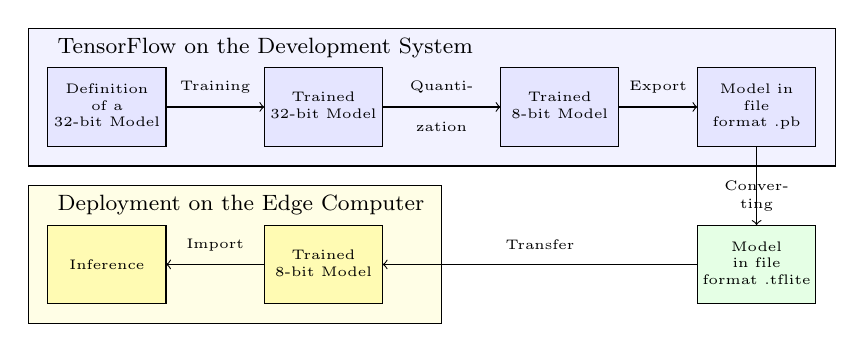
\begin{tikzpicture}
    
  \draw[fill=blue!5] (-0.25,-0.25) -- (10,-0.25) -- (10,1.5) -- (-0.25,1.5) -- cycle;
  \draw[fill=blue!10] (0,0) -- (1.5,0) -- (1.5,1) -- (0,1) -- cycle;
  \node[right] (TF) at (0.0,1.25) {\footnotesize TensorFlow on the Development System};
  
  \node (T32) at (0.75,0.5) {\tiny \begin{tabular}{c} Definition\\ of a \\ 32-bit Model\\ \end{tabular}};
  
  \node (T32) at (2.125,0.75) {\tiny Training};
  \draw[->] (1.5,0.5) -- (2.75,0.5);
  \draw[fill=blue!10] (2.75,0) -- (4.25,0) -- (4.25,1) -- (2.75,1) -- cycle;
  \node (T32) at (3.5,0.5) {\tiny \begin{tabular}{c}  Trained\\ 32-bit Model\\ \end{tabular}};
  
  \node (T32) at (5.0,0.75) {\tiny Quanti-};
  \node (T32) at (5.0,0.25) {\tiny zation};
  \draw[->] (4.25,0.5) -- (5.75,0.5);
  \draw[fill=blue!10] (5.75,0) -- (7.25,0) -- (7.25,1) -- (5.75,1) -- cycle;
  \node (T32) at (6.5,0.5) {\tiny \begin{tabular}{c} Trained\\ 8-bit Model\\ \end{tabular}};

  \node (T32) at (7.75,0.75) {\tiny Export};
  \draw[->] (7.25,0.5) -- (8.25,0.5);
  \draw[fill=blue!10] (8.25,0) -- (9.75,0) -- (9.75,1) -- (8.25,1) -- cycle;
  \node (T32) at (9,0.5) {\tiny \begin{tabular}{c} Model in \\ file \\format .pb\\ \end{tabular}};

  \node (T32) at (9,-0.5) {\tiny Conver- };
  \node (T32) at (9,-0.75) {\tiny ting};
  \draw[->] (9,0) -- (9,-1);
  \draw[fill=green!10] (8.25,-1) -- (9.75,-1) -- (9.75,-2) -- (8.25,-2) -- cycle;
  \node (T32) at (9,-1.5) {\tiny \begin{tabular}{c} Model \\in file \\ format .tflite \\ \end{tabular}};

  
  \draw[fill=yellow!10] (-0.25,-0.5) -- (5.0,-0.5) -- (5.0,-2.25) -- (-0.25,-2.25) -- cycle;
  \node[right] (T32) at (0.0,-0.75) {\footnotesize Deployment on the Edge Computer};
  \node (T32) at (6.25,-1.25) {\tiny Transfer};
  \draw[<-] (4.25,-1.5) -- (8.25,-1.5);
  \draw[fill=yellow!30] (2.75,-1) -- (4.25,-1) -- (4.25,-2) -- (2.75,-2) -- cycle;

   \node (T32) at (3.5,-1.5) {\tiny \begin{tabular}{c} Trained\\ 8-bit Model\\ \end{tabular}};

  \node (T32) at (2.125,-1.25) {\tiny Import};
  \draw[<-] (1.5,-1.5) -- (2.75,-1.5);
  \draw[fill=yellow!30] (0,-1) -- (1.5,-1) -- (1.5,-2) -- (0,-2) -- cycle;
   \node (T32) at (0.75,-1.5) {\tiny Inference};

\end{tikzpicture}  
  
%    \includegraphics[width=0.7\textwidth]{Software/flowchart} 
    
    \captionof{figure}{The basic process for creating a model for an edge computer \cite{GoogleTensorFlowModel:2019}}\label{Software:Flowchart}

\end{center}


\Mynote{Where are these steps explained?}


\section{TensorFlow Lite: Tool and Libraries}

TensorFlow Lite is a name for a tool, the TensorFlow Lite Converter, and a name for a library.
Both types are eplained in the following subsections.

\subsection{TensorFlow Lite as a Library in TensorFlow}


\subsubsection{Model Creation and Training}
The first step involves creating and training a machine learning model using TensorFlow. 
\\TensorFlow Lite uses TensorFlow models converted into a smaller, more efficient machine learning (ML) model format. You can use pre-trained models with TensorFlow Lite, modify existing models, or build your own TensorFlow models and then convert them to TensorFlow Lite format. TensorFlow Lite models can perform almost any task a regular TensorFlow model can do: object detection, natural language processing, pattern recognition, and more using a wide range of input data including images, video, audio, and text

\subsubsection{Model Conversion}
Once the model is trained, it needs to be converted into a TensorFlow Lite model. The TensorFlow Lite converter takes a TensorFlow model and generates a TensorFlow Lite model, an optimized FlatBuffer format identified by the file extension \FILE{.tflite}.

The model conversion can be done using the Python API or the Command
line tool
\begin{itemize}
    \item Command-line Tool: \SHELL{tflite convert}
    \item Python API: \SHELL{tf.lite.TFLiteConverter}
\end{itemize}

The process involves several steps:
\begin{itemize}
    \item \textbf{Select the Model}: The converter accepts the following input model formats.
    \begin{itemize}
        \item \FILE{SavedModel}: A TensorFlow model saved as a set of files on disk.
        \item \FILE{Keras model}: A model created using the high level Keras API.
        \item \FILE{Keras H5 format}: A light-weight alternative to SavedModel format supported by Keras API.
        \item \FILE{Models built from concrete functions}: A model created using the low level TensorFlow API.
    \end{itemize}
    
    \item \textbf{Optimize the Model}: During conversion, various optimization techniques can be applied to make the model more efficient. These include:
    \begin{itemize}
        \item \textbf{Post-training Quantization}: Reduces the model size and improves latency by converting floating-point numbers to more efficient lower precision numbers like 8-bit integers.
        \item \textbf{Pruning}: Reduces the number of operations in a model by removing redundant connections. This helps in decreasing the model size and improving inference speed.
        \item \textbf{Clustering}: Groups similar model weights together to make the model more efficient during computation, which can lead to faster inference and reduced model size.
    \end{itemize}
\end{itemize}

The goal of these optimizations is to make the model smaller and faster while maintaining accuracy.

\subsubsection{Model Deployment}
After converting the model to a file \FILE{.tflite}, it can be deployed on a variety of devices including mobile phones, embedded systems, and microcontrollers. TensorFlow Lite supports deployment on both Android and iOS platforms, as well as other systems like Arduinox.

\subsubsection{Running Inference}
To run inference with TensorFlow Lite, you need to use the TensorFlow Lite Interpreter. Here’s the typical process:
\begin{itemize}
    \item \textbf{Load the Model}: The TensorFlow Lite model file \FILE{.tflite} is loaded into the memory, which contains the model's execution graph
    \item \textbf{Allocate Tensors}: Memory is allocated for the input and output tensors.
    \item \textbf{Set Input Data}: The input data is preprocessed and fed into the model.
    \item \textbf{Invoke the Interpreter}: The interpreter runs the model with the input data to produce the output.
    \item \textbf{Get Output Data}: The output data is extracted and post-processed to get the final predictions.
\end{itemize}

% Include a specific range of lines from the Python file for InterfaceCode
\lstinputlisting[language=Python, firstline=1, lastline=17]{../../Code/TensorFlowLite/InterfaceCode.py}

\subsubsection{Tensors in TensorFlow Lite}
In TensorFlow Lite, a tensor is a multi-dimensional array that represents the basic data structure used by the library. Just like a vector is a one-dimensional array and a matrix is a two-dimensional array, a tensor can be n-dimensional. Tensors can have different shapes and data types, and they are used for both input and output of the model. Here's a brief overview of tensors:

\begin{itemize} 
    
    \item \textbf{Shape}: The shape of a tensor defines the number of elements in each dimension. For example, a tensor with shape [2, 3, 4] has 2 elements in the first dimension, 3 elements in the second dimension, and 4 elements in the third dimension.
    
    \item \textbf{Data Type}: Tensors can contain different types of data, such as integers, floating-point numbers, or strings. The data type is specified when the tensor is created.
    
    \item \textbf{Usage in TensorFlow Lite}:
    \begin{itemize}
        \item \textbf{Input Tensors}: These are used to feed the input data into the model. The input tensor shape and data type must match what the model expects.
        \item \textbf{Output Tensors}: These store the results produced by the model after running inference. The output tensor shape and data type depend on the model's architecture and the specific task it performs.
    \end{itemize}
\end{itemize}

\textbf{Example}:
\begin{itemize}
    \item If a model expects an input image of size 224x224 with 3 color channels (RGB), the input tensor shape might be [1, 224, 224, 3], where 1 represents the batch size. After running inference, the output might be a tensor of shape [1, 1000] if the model outputs probabilities for 1000 different classes.
    \item If an object detection model processes an input image of size 300x300 with 3 color channels (RGB), the input tensor shape might be [1, 300, 300, 3]. The output tensor might include bounding boxes, with a shape of [1, 10, 4] where 10 represents the number of detected objects and 4 represents the coordinates of each bounding box.
\end{itemize}


\subsubsection{Optimization Techniques}
TensorFlow Lite supports various optimization techniques to enhance the performance and efficiency of models on edge devices:
\begin{itemize}
    \item \textbf{Quantization}: Converts high precision numbers to lower precision numbers, which reduces model size and improves latency.
    \item \textbf{Delegates}: Uses hardware acceleration to run models more efficiently. TensorFlow Lite supports GPU and NNAPI delegates among others.
    \item \textbf{Pruning}: Reduces the number of operations and model size by removing unnecessary weights. Pruning simplifies the model, which can lead to improved inference speed and reduced memory usage.
    \item \textbf{Clustering}: Involves grouping similar weights in a model, reducing the number of unique weight values. This process makes the model more efficient during computation, which can lead to faster inference and smaller model size.
\end{itemize}

These optimizations make TensorFlow Lite models suitable for deployment in resource-constrained environments while maintaining performance and accuracy.




\subsection{TensorFlow Lite Converter}

The TensorFlow Lite Converter is a tool available as a Python API that converts trained TensorFlow models into the TensorFlow Lite format. This is done by converting the Keras model into the form of a FlatBuffer, a special space-saving file format. In general, converting models reduces file size and introduces optimisations without compromising accuracy. The TensorFlow Lite converter continues to offer options to further reduce file size and increase execution speed, with some trade-offs in accuracy. \cite{Google.09.10.2020,Warden:2020}

\Mynote{How does it work?\\
    \begin{itemize}
    \item Installation
    \item use
    \item syntax
    \item examples
\end{itemize}
}

One way to optimise is quantisation. While the weights of the models are usually stored as 32-bit floating point numbers, they can be converted to 8-bit integers with only a minimal loss in the accuracy of the model. This saves memory and also allows for faster computation, as a \ac{cpu} works more efficiently with integers. \cite{Warden:2020}


\subsubsection{Installation procedure}

\begin{itemize}
    \item Install the latest version of Python using the following link \url{https://www.python.org/downloads/}
    \item \textbf{pip} is the package installer for Python. It should be installed by default with Python
    \item TensorFlow can be installed using pip. Open Command Prompt or PowerShell and run \SHELL{pip install tensorflow} ~\ref{GoogleTensorFlowInstall:2019}
    \item To verify the installation, open a Python shell and type \SHELL{python} and import TensorFlow by typing \SHELL{import tensorflow as tf
    }, after importing TensorFlow, you can check the version using  \SHELL{print(tf.\_\_version\_\_)} ~\ref{TflVersion} \cite{GoogleTensorFlowInstall:2019}
\end{itemize}

\begin{figure}
    \begin{center}
        
\includegraphics[width=0.7\linewidth]{TensorFlowLite/TensorFlowInstallation.png}
        \caption{TensorFLow Lite Installation on PC}
        \label{TflInstallation}
    \end{center}
\end{figure}

\begin{figure}
    \begin{center}
        
\includegraphics[width=0.7\linewidth]{TensorFlowLite/TensorFlowVersion.png}
        \caption{TensorFLow Lite Version}
        \label{TflVersion}
    \end{center}
\end{figure}

\subsubsection{Example Program}

\begin{enumerate}
    \item Training a simple model capable of performing simple arithmetic addition of two input numbers using TensorFlow. Run the model in python to generate the file \FILE{addition\_model.h5} in the same directory of tensorflow model. ~\ref{lst:SimpleModel}
    
    % Python file for Simple Model
    \lstinputlisting[language=Python, firstline=1, lastline=28, caption={Simple TensorFlow Model}, label={lst:SimpleModel}]{../../Code/TensorFlowLite/SimpleModel.py}
    
    
    \item Convert the Keras Model to TensorFlow Lite using the python script in the same directory and run the command \PYTHON{python convertModelTotflite.py} in command prompt.  ~\ref{lst:ModelConversion}
    
    % 
    \lstinputlisting[language=Python, firstline=1, lastline=19, caption={Python script for Model convertion to TensorFlow Lite}, label={lst:ModelConversion}]{../../Code/TensorFlowLite/ModelConversion.py}
    
    \item Using the python script convert the TensorFlow Lite Model to a C Array and run the python \PYTHON{ConvertTfliteToHeader.py} in the command prompt.  ~\ref{lst:TFLtoCArray}
    
    % 
    \lstinputlisting[language=Python, firstline=1, lastline=34, caption={Python Script to TensorFlow Lite Model into C Array}, label={lst:TFLtoCArray}]{../../Code/TensorFlowLite/TFLtoCArray.py}
    
    
    \item Now include the model in the Arduino Sketch ~\ref{ArduinoSketch} and run it on the Arduino board and interact with serial monitor to see the result. ~\ref{lst:ArduinoSketch}
    
    % 
    \lstinputlisting[language=C++, firstline=1, lastline=45, caption={Arduino Sketch to run the model}, label={lst:ArduinoSketch}]{../../Code/TensorFlowLite/ArduinoSketch.cpp}
    
    
\end{enumerate}






\subsection{TensorFlow Lite as a Library in the Arduino IDE}

The TensorFlow Lite interpreter is a library that executes an appropriately converted TensorFlow Lite model using the most efficient operations for the given device, applying the operations defined in the model to the input and providing access to the output. It works across platforms and provides a simple API to run TensorFlow Lite models from Java, Swift, Objective-C, C ++ and Python.\cite{Google.09.10.2020,Warden:2020}

To use hardware acceleration on different devices, the TensorFlow Lite interpreter can be configured with \glqq delegates\grqq. These use device accelerators such as an \ac{gpu} or a digital signal processor (DSP). \cite{Google.09.10.2020}

\subsubsection{Introduction}

TensorFlow was composed of three parts tool, training and library. The library is one part of TensorFlow Lite. 

On this part we saw the library who was used for the magic wand project.

The library was composed of different headler files, a headler file is a file type used for interface declaration, redundancy prevention, inclusion in the source file, separation of interface and implementation and protection against multiple inclusion. 
The explanation of the library TensorFlow Lite needed some resource, we can found part of this on TensorFlow website. \cite{GoogleTensorFlowAPI:2023}

\bigskip

On this example of Magic Wand, we have this headler files : 

\begin{itemize}
    \item \FILE{tensorflow/lite/kernels/micro\_ops.h}
    \item \FILE{tensorflow/lite/micro/micro\_error\_reporter.h}
    \item \FILE{tensorflow/lite/micro/micro\_mutable\_op\_resolver.h}
    \item \FILE{tensorflow/lite/micro/micro\_interpreter.h}
    \item \FILE{tensorflow/lite/c/common.h}
    \item \FILE{tensorflow/lite/core/api/op\_resolver.h}
    \item \FILE{tensorflow/lite/micro/compatibility.h}
    \item \FILE{tensorflow/lite/schema/schema\_generated.h}
\end{itemize}

\subsubsection{File \FILE{micro\_ops.h}}

\begin{center}
    \captionof{code}{Micro Opération}
    \ArduinoExternal{firstline=15,lastline= 24 }{../../Code/Arduino/TensorFlowLite/src/tensorflow/lite/micro/kernels/micro_ops.h}
    \label{MicroOps}
\end{center}

The first part of the document was used to check if  TENSORFLOW\_LITE\_MICRO\_KERNELS\_MICRO\_OPS\_H\_ was define, if it was define the programme go to \PYTHON{\#endif}. If it wasn't the programme run and do : 

\begin{itemize}
    \item \PYTHON{\#define} TENSORFLOW\_LITE\_MICRO\_KERNELS\_MICRO\_OPS\_H\_ : this is the fucntion check. 
    \item namespace tflite {namespace ops {namespace micro {text}}} : 
    \item 'text' is representation of alll \PYTHON{TfLiteRegistration * Register\_function}  : this subspace allows you to define a specific path for the \PYTHON{TfLiteRegistration\* Register\_function()}, \PYTHON{TfLIteRegistration} can handle the function() while \PYTHON{ * } sets a pointer. \PYTHON{Register} is a function for registering the function. The regestried function is define with the code \ref{Figure:RegistredFunction}.
\end{itemize} 

\begin{center}
    \captionof{code}{Function Register}
    \ArduinoExternal{firstline=31, lastline=80}{../../Code/Arduino/TensorFlowLite/src/tensorflow/lite/micro/kernels/micro_ops.h}
    \label{Figure:RegistredFunction}
\end{center}


\subsubsection{File \FILE{micro\_error\_reporter.h}}

The file begin by check is TENSORFLOW\_LITE\_MICRO\_ERROR\_REPORTER\_H\_ was define, if it was define the programme run to \PYTHON{\#endif}. If it wasn't define it programme run. 

It define TENSORFLOW\_LITE\_MICRO\_ERROR\_REPORTER\_H\_. 
It include 4 files : 

\begin{itemize}
    \item \FILE{tensorflow/lite/core/api/error\_reporter.h}
    \item \FILE{tensorflow/lite/micro/compatibility.h}
    \item \FILE{tensorflow/lite/micro/debug\_log.h}
    \item \FILE{tensorflow/lite/micro/debug\_log\_numbers.h}
\end{itemize}

It create a namespace named tflite, this space have class MicroErrorReporter and it was public. A function was created it's was a integer function and his name is Report it depend by \PYTHON{const char} * format, va\_list args.
A new value was create it's TF\_LITE\_REMOVE\_VIRTUAL\_DELETE, it was a private value. 

\begin{center}
    \captionof{code}{Function Micro Error Reporter}
    \ArduinoExternal{firstline=15}{../../Code/Arduino/TensorFlowLite/src/tensorflow/lite/micro/micro_error_reporter.h}
    \label{Figure:MicroErrorRep}
\end{center}

\subsubsection{File \FILE{micro\_mutable\_op\_resolver.h}}

The file begin by check is TENSORFLOW\_LITE\_MICRO\_MUTABLE\_OP\_RESOLVER\_H\_ was define, if it was define the programme run to \PYTHON{\#endif}. If it wasn't define it programme run. 

\begin{itemize}
    \item \FILE{tensorflow/lite/c/common.h}
    \item \FILE{tensorflow/lite/core/api/op\_resolver.h}
    \item \FILE{tensorflow/lite/micro/compatibility.h}
    \item \FILE{tensorflow/lite/schema/schema\_generated.h}
\end{itemize}

They define the function \PYTHON{TFLITE\_REGISTRATIONS\_MAX(128)} 

\begin{center}
    \captionof{code}{Function Micro OP Solver}
    \ArduinoExternal{firstline=15, lastline=26}{../../Code/Arduino/TensorFlowLite/src/tensorflow/lite/micro/micro_mutable_op_resolver.h}
    \label{Figure:MicroErrorRep}
\end{center}	

A new space who was a under function of tflite as create. 
The class \PYTHON{templace} set on tOpCount value and TFLITE\_REGISTRATIONS\_MAX is the maximum value who MicroOpResolver can solve. 

public return \PYTHON{TfLiteRegistration} who have parameter \PYTHON{op} and \PYTHON{version}. The FindOp overchage method of the OpResolver class.

The function \PYTHON{registration} is a chart of TfLiteRegistration and he can save data,\PYTHON{registrations\_len\_} is the lenght of the file.

If the registration builtin code is equivalent to op and the version is the same so they return the pointer of registration. 
And they return nullotr at the end of for loop. 

\begin{center}
    \captionof{code}{Function Micro OP Solver}
    \ArduinoExternal{firstline=27, lastline=45}{../../Code/Arduino//TensorFlowLite/src/tensorflow/lite/micro/micro_mutable_op_resolver.h}
    \label{Figure:MicroErrorRep}
\end{center}

The const \PYTHON{TfLiteRegistration} who have pointer with parameter \PYTHON{op} and \PYTHON{version}. The \PYTHON{override} used loop \PYTHON{for} and it check 3 conditions. 

\begin{itemize}
    
    \item registration.builtin\_code == BuiltinOperator\_CUSTOM check about operation in code is personalized. 
    \item (strcmp(registration.custom\_name, op) == 0 check if the name is the same. 
    \item registration.version is same with version
    
\end{itemize}
If the 3 condition is okay, it return registration. 

\begin{center}
    \captionof{code}{Function Micro OP Solver}
    \ArduinoExternal{firstline=46, lastline=58}{../../Code/Arduino//TensorFlowLite/src/tensorflow/lite/micro/micro_mutable_op_resolver.h}
    \label{Figure:MicroErrorRep}
\end{center}

The function \PYTHON{AddBuiltin} have pointer on registration and depend of BuiltinOperator op, and set the minimal and maximal version at 1. 

If the function AddBuiltin is call they do this function one time. 

It do a pointer on new\_registation and it choice the statement avaible on registration. The lenght up by one for new register. 

The registration value is put on new\_registration and the builtin\_code value is change for op, the new\_registration version is change to version.  

\begin{center}
    \captionof{code}{Function Micro OP Solver}
    \ArduinoExternal{firstline=59, lastline=74}{../../Code/Arduino//TensorFlowLite/src/tensorflow/lite/micro/micro_mutable_op_resolver.h}
    \label{Figure:MicroErrorRep}
\end{center}

The function \PYTHON{AddCustom} have pointer on registration and depend of BuiltinOperator op, and set the minimal and maximal version at 1. 



It do a pointer on new\_registation and it choice the statement avaible on registration. The lenght up by one for new register. 

The registration value is put on new\_registration and the builtin\_code value is change for op, the new\_registration version is change to version.  

\begin{center}
    \captionof{code}{Function Micro OP Solver}
    \ArduinoExternal{firstline=76, lastline=92}{../../Code/Arduino//TensorFlowLite/src/tensorflow/lite/micro/micro_mutable_op_resolver.h}
    \label{Figure:MicroErrorRep}
\end{center}

To \PYTHON{GetRegistrationLenght()} return registration\_len. 

The chart TfLiteRegistration[ ] save tOpCount data. The registrations\_len was change on 0 and \PYTHON{TF\_LITE\_REMOVE\_VIRTUAL\_DELETE} deactivates the virtual destructor of class. 

The class \PYTHON{MicroMutableOpResolver} was public and have the parameter \PYTHON{TFLITE\_REGISTRATIONS\_MAX}. The virtual destructor of class was desactivates.

\begin{center}
    \captionof{code}{Function Micro OP Solver}
    \ArduinoExternal{firstline=93}{../../Code/Arduino//TensorFlowLite/src/tensorflow/lite/micro/micro_mutable_op_resolver.h}
    \label{Figure:MicroErrorRep}
\end{center}


\subsubsection{File \FILE{micro\_interpreter.h}}

The file begin by check is TENSORFLOW\_LITE\_MICRO\_MICRO\_INTERPRETER\_H\_ was define, if it was define the programme run to \PYTHON{\#endif}. If it wasn't define it programme run. 

It define TENSORFLOW\_LITE\_MICRO\_MICRO\_INTERPRETER\_H\_. 
It include 4 files : 

\begin{itemize}
    \item \FILE{tensorflow/lite/c/common.h}
    \item \FILE{tensorflow/lite/core/api/error\_reporter.h}
    \item \FILE{tensorflow/lite/core/api/op\_resolver.h}
    \item \FILE{tensorflow/lite/kernels/internal/tensor\_ctypes.h}
    \item \FILE{tensorflow/lite/micro/micro\_allocator.h}
    \item \FILE{tensorflow/lite/schema/schema\_generated.h}
    \item \FILE{tensorflow/lite/type\_to\_tflitetype.h}
\end{itemize}

\begin{center}
    \captionof{code}{Function Micro OP Solver}
    \ArduinoExternal{firstline=15, lastline=25}{../../Code/Arduino//TensorFlowLite/src/tensorflow/lite/micro/micro_interpreter.h}
    \label{Figure:MicroErrorRep}
\end{center}


It define class \PYTHON{MicroInterpreter}, \PYTHON{MicroInterpreter} take different value, it have pointer  model for machine learning, op\_resolver was solve operation, tensor\_arena who save data, tensor\_arena\_size define the size avec tensor\_arena and error\_reporter have pointer look ErrorReporter. 


\begin{center}
    \captionof{code}{Function Micro OP Solver}
    \ArduinoExternal{firstline=27, lastline=43}{../../Code/Arduino//TensorFlowLite/src/tensorflow/lite/micro/micro_interpreter.h}
    \label{Figure:MicroErrorRep}
\end{center}

Memory was given to \PYTHON{AllocateTensors()} and also to \PYTHON{Invoke()}.The tensor\_size of size\_t depend with context\_. The TfLiteTensor * pointer on tensor\_index. 

The pointer of tensor\_ptr try to read data of pointer on tensor\_index and if it read it do the second loop for. The second loop check the type fo tensor if it's the same  with \PYTHON{typeToTfLiteType<T>()} and if it's it return GetTensorData<T>(tensor\_ptr).

\begin{center}
    \captionof{code}{Function Micro OP Solver}
    \ArduinoExternal{firstline=46, lastline=63}{../../Code/Arduino//TensorFlowLite/src/tensorflow/lite/micro/micro_interpreter.h}
    \label{Figure:MicroErrorRep}
\end{center}

TfLiteTensor return to specific and it return to size\_t index. The \PYTHON{size\_t inputs\_size()} and he was return by the value of size lenght on the subgraph.

The \PYTHON{flatbuffers::Vector<int32\_t>\& inputs()} return value on pointer. 

TfLiteTensor * take a pointer of \PYTHON{input\_tensor} and on his argument size\_t index and it return the value on \PYTHON{input(index)}.
A pointer of T class on typed\_input\_tensor (tensor\_index).On his function we have two 'if' loops, each of which contains a condition. 
THe first one is the pointer on \PYTHON{tensor\_ptr} is egal with \PYTHON{input\_tensor(tensor\_index)} and it return value of \PYTHON{GetTensorData<T>(tesnor\_ptr)}.

\begin{center}
    \captionof{code}{Function Micro OP Solver}
    \ArduinoExternal{firstline=65, lastline=79}{../../Code/Arduino//TensorFlowLite/src/tensorflow/lite/micro/micro_interpreter.h}
    \label{Figure:MicroErrorRep}
\end{center}

The create a pointer type * in \PYTHON{output(size\_t index)}.The \PYTHON{size\_t outputs\_size()} and return the lenght of subgraph. 
The  value of \PYTHON{flatbuffers::Vector<int32\_t>} depend of int32\_t values and the value return depend off pointer subgraph\_ on output. 

A pointer of T class on typed\_input\_tensor (tensor\_index).On his function we have two 'if' loops, each of which contains a condition. 
THe first one is the pointer on \PYTHON{tensor\_ptr} is egal with \PYTHON{input\_tensor(tensor\_index)} and it return value of \PYTHON{GetTensorData<T>(tesnor\_ptr)}.

\begin{center}
    \captionof{code}{Function Micro OP Solver}
    \ArduinoExternal{firstline=81, lastline=95}{../../Code/Arduino//TensorFlowLite/src/tensorflow/lite/micro/micro_interpreter.h}
    \label{Figure:MicroErrorRep}
\end{center}


A new variable as created it's a \PYTHON{ResetVaraibleTensor()}. 

A new variable as created it's a \PYTHON{intialization\_status()} and return initialization\_status\_. 
A pointer type ErrorReporter name error\_reporter() retunr error\_reporter\_. 

size\_t \PYTHON{operators\_size()} was used to return the size of operators. 

A part of the project was used for only debugging. 

The type of object is NodeAndRegistration and the function name \PYTHON{node\_and\_registration}, the function depend of node\_index argument. It retunr \PYTHON{node\_and\_registrztion[node\_index]}.

\begin{center}
    \captionof{code}{Function Micro OP Solver}
    \ArduinoExternal{firstline=98, lastline=109}{../../Code/Arduino//TensorFlowLite/src/tensorflow/lite/micro/micro_interpreter.h}
    \label{Figure:MicroErrorRep}
\end{center}
The \PYTHON{private} part was used to separate to part of code function. 

The function \PYTHON{CorrectTensorEndianness<} depedn of (TfLiteTensor * tensorCorr)

A nex class was created, it's T class.The function \PYTHON{CorrectTensorDataEndianness} depend of T * data and int32\_t size. Differenet fucntion was created, we have : 

\begin{itemize}	
    \item Model * do a pointer type * on \PYTHON{model\_}
    \item OpResolver\&  is a constant reference on \PYTHON{op\_resolver\_}
    \item ErrorReporter * is a pointer type ErrorReporter on \PYTHON{error\_reporter\_}
    \item \PYTHON{context\_} is on TfLiteContext type and it was initialize with default value. 
    \item \PYTHON{allocator\_} is type MicroAllocator and it was used to allocate and manage memory at runtime.
    \item \PYTHON{tensors\_allocated\_} is bool and check is tensor is allocated or non. 
    \item \PYTHON{initializatio\_status\_ }is on type TfLiteStatus
    \item A point type SubGraph was used on \PYTHON{subgraph\_}
\end{itemize}

The const \PYTHON{flatbuffers::Vector<flatbuffers::Offset<Tensor>>* tensors\_} come of FlatBuffer library and the pointer can't change of  target after loading and it point of tensor\_. It have data type Tensor. 

The const \PYTHON{flatbuffers::Vector<flatbuffers::Offset<Operator>> * operator\_} come of FlatBuffer library and the pointer check on operator\_ can't change of  target after loading. It have data type Operator. 

\begin{center}
    \captionof{code}{Function Micro OP Solver}
    \ArduinoExternal{firstline=111, lastline=135}{../../Code/Arduino//TensorFlowLite/src/tensorflow/lite/micro/micro_interpreter.h}
    \label{Figure:MicroErrorRep}
\end{center}

\subsubsection{File \FILE{c\_common.h}}

The file begin by check is TENSORFLOW\_LITE\_C\_COMMON\_H\_ was define, if it was define the programme run to \PYTHON{\#endif}. If it wasn't define it programme run. It include 3 libraries : 

\begin{itemize}
    \item \FILE{stdbool.h} used for include boolean on C
    \item \FILE{stddef.h} used to define new macro and type 
    \item \FILE{stdint.h} used to  give definitions for fixed-size integer types
\end{itemize}

It check if \_\_cplusplus is define and print \textcolor{violet}{"C"}.

It declare typedef  for new enumeration named \PYTHON{TfLiteStatus},  we have kTfLiteOk = 0 and kTfLiteError = 1 and TfLiteStatus was used for an alias. 

\begin{center}
    \captionof{code}{Function common}
    \ArduinoExternal{firstline=33, lastline=45}{../../Code/Arduino//TensorFlowLite/src/tensorflow/lite/c/common.h}
    \label{Figure:Comatibily}
\end{center}

We have a enumeration of the function
\PYTHON{TfLiteExternalContextType} this enumeration is composed by : 

\begin{enumerate}	
    \item kTfLiteEigenContext = 0 and this is a library Eigen in C++ for matrix calculation.
    \item kTfLiteGemmLowpContext = 1 it was used for library \FILE{gemm\_support.h} for low-precision matrix-matrix product operations.
    \item kTfLiteEdgeTpuContext = 2 is for support the Edge TPU, a hardware acceleration chip for neural network inference on the device.
    \item kTfLiteCpuBackendContext = 3, this file \FILE{cpu\_backend\_support.h} is used for running on CPU
    \item kTfLiteCpuBackendContext = 3
    \item kTfLiteMaxExternalContexts = 4 it was used for the maximum number of external contexts available.
\end{enumerate}

We define 3 structure: 
\begin{itemize}
    \item TfLiteContext, in general this structure is used to group differenet variable. 
    \item TfLiteContex, in general this is used to do optimisation on the library and system. 
    \item TfLiteRegistration is used on initialization and execution functions, input and output tensor types. 
\end{itemize}

\begin{center}
    \captionof{code}{Function common}
    \ArduinoExternal{firstline=50, lastline=62}{../../Code/Arduino//TensorFlowLite/src/tensorflow/lite/c/common.h}
    \label{Figure:Comatibily}
\end{center}

It define a function structure \PYTHON{TfLiteExternalContext}. It create function TfLiteExternalContextType with \PYTHON{TfLiteExternalContext}, it create pointer with basic point TfLiteExternalContext, the pointer is on Refresh and reffered to TfLiteStatus. 

A macro name kTfLiteOptionalTensor(-1)  was define. A structure was define and name TfiteIntArray witch depend a integer value \PYTHON{size}.

The \PYTHON{\#if} is like if but it was check before the program run. It \#if have 4 conditions : 

\begin{itemize}
    \item \PYTHON{!defined(\_\_clang\_\_)}: This part checks if \_\_clang\_\_ is not defined. If it's defined when the code is compiled with the Clang compiler.  This part of the code ensures that the code will not be included if the compiler used is not Clang.
    
    \item \PYTHON{defined(\_\_GNUC\_\_)}: This checks whether the \_\_GNUC\_\_ symbol is defined. If it's defined when the code is compiled with the GCC (GNU Compiler Collection) compiler. This part of the code verifies that the compiler used is GCC.
    
    \item \PYTHON{\_\_GNUC\_\_ == 6} : This checks whether the main version of the GCC compiler is version 6.
    
    \item \PYTHON{\_\_GNUC\_MINOR\_\_ >= 1}: This checks whether the minor version of the GCC compiler is greater than or equal to 1, with the GCC version 6.1 or later.
\end{itemize}

If the 4 conditions is here, it create data char with  size of 0 else it create char but don't define this size. 

\begin{center}
    \captionof{code}{Function common}
    \ArduinoExternal{firstline=69, lastline=88}{../../Code/Arduino//TensorFlowLite/src/tensorflow/lite/c/common.h}
    \label{Figure:Comatibily}
\end{center}
The \PYTHON{TfLiteIntArrayGetSizeInBytes} was use to givethe precise size of chart.  

A macro name TF\_LITE\_STATIC\_MEMORY is check. If it's not define it create structure TfLiteIntArray for manage integer arrays and the size of chart is size. 

The function \PYTHON{TfLiteIntArrayEqual} compares two integer arrays TfLiteIntArray and returns 1 (true) if it are equal, i.e. if it have the same length and the same elements, otherwise it returns 0 (false).


The function \PYTHON{TfLiteIntArrayEqualsArray} compares an integer array TfLiteIntArray with a conventional integer array b\_data of size b\_size, and returns 1 (true) if it are of the same length and contain the same elements, otherwise it returns 0 (false).


The program check if the macro \PYTHON{TF\_LITE\_STATIC\_MEMORY} is define. If it's define it go to \#endif. 

The function \PYTHON{TfLiteIntArrayCopy} creates a copy of a source(src) TfLiteIntArray integer array and returns a pointer to this new copy. This allows you to duplicate the data in the array without modifying the original.

The function \PYTHON{TfLiteIntArrayFree} frees the memory allocated for an integer array TfLiteIntArray (a). This prevents memory leaks by ensuring that unused memory is properly returned to the system.


A structure name \PYTHON{TfLiteFloatArray} is define and define a size on int. 

\begin{center}
    \captionof{code}{Function common}
    \ArduinoExternal{firstline=92, lastline=118}{../../Code/Arduino//TensorFlowLite/src/tensorflow/lite/c/common.h}
    \label{Figure:Comatibily}
\end{center}

The \PYTHON{\#if} is like if but it was check before the program run. It \#if have 4 conditions : 

\begin{itemize}
    \item \PYTHON{!defined(\_\_clang\_\_)}: This part checks if \_\_clang\_\_ is not defined. If it's defined when the code is compiled with the Clang compiler.  This part of the code ensures that the code will not be included if the compiler used is not Clang.
    
    \item \PYTHON{defined(\_\_GNUC\_\_)}: This checks whether the \_\_GNUC\_\_ symbol is defined. If it's defined when the code is compiled with the GCC (GNU Compiler Collection) compiler. This part of the code verifies that the compiler used is GCC.
    
    \item \PYTHON{\_\_GNUC\_\_ == 6} : This checks whether the main version of the GCC compiler is version 6.
    
    \item \PYTHON{\_\_GNUC\_MINOR\_\_ >= 1}: This checks whether the minor version of the GCC compiler is greater than or equal to 1, with the GCC version 6.1 or later.
\end{itemize}

If the 4 conditions is here, it create data char with  size of 0 else it create char but don't define this size. 

A function \PYTHON{TfLiteFloatArrayGetSizeInBytes} depending on size. 

The program check if the macro \PYTHON{TF\_LITE\_STATIC\_MEMORY} is define. If it's define it go to \#endif. 

The function \PYTHON{TfLiteFloatArrayCreate} allocates memory for a float array TfLiteFloatArray of size size and returns a pointer to this new array.This initializes an array for storing floating-point numbers.

The function \PYTHON{TfLiteFloatArrayFree} frees the memory allocated for a TfLiteFloatArray (a) float array. This prevents memory leaks by ensuring that allocated memory is properly returned to the system once the array is no longer required.

\begin{center}
    \captionof{code}{Function common}
    \ArduinoExternal{firstline=121, lastline=140}{../../Code/Arduino//TensorFlowLite/src/tensorflow/lite/c/common.h}
    \label{Figure:Comatibily}
\end{center}

The program check if the macro \PYTHON{TF\_LITE\_STRIP\_ERROR\_STRINGS} is define. If it's define it go to \#else.If it wasn't define it define macro  \PYTHON{TF\_LITE\_KERNEL\_LOG}.

The macro encapsulated in a do-while (false) loop executes the ReportError command from the context, passing the context and other variable arguments. This structure ensures that the call to ReportError behaves as a single instruction, even if it contains commas, so that it can be used safely in the program.  The use of \_\_VA\_ARGS\_\_ allows you to pass a variable number of arguments to the ReportError function.


The macro \PYTHON{TF\_LITE\_ENSURE\_MSG(context, value, msg)} is define. The loop do{}while(0) is alway doing one time. It uses \PYTHON{TF\_LITE\_KERNEL\_LOG} to log an error message, which includes the source file name (\_\_FILE\_\_) and the specified message (msg) and returns kTfLiteError, indicating an error. 

\begin{center}
    \captionof{code}{Function common}
    \ArduinoExternal{firstline=149, lastline=166}{../../Code/Arduino//TensorFlowLite/src/tensorflow/lite/c/common.h}
    \label{Figure:Comatibily}
\end{center}


The macro \PYTHON{TF\_LITE\_ENSURE(context, a)} is define 
This loop is doing one time. If a is not true, it register error message composed by \textcolor{violet}{FILE : LINE, FILE was not true} and it return showing an error. 

\bigskip

The macro \PYTHON{TF\_LITE\_ENSURE\_STATUS(a)} is define. 
This loop is doing one time. If a is different with kTfLiteOk, it  return showing an error. 

\begin{center}
    \captionof{code}{Function commom}
    \ArduinoExternal{firstline=170, lastline=184}{../../Code/Arduino//TensorFlowLite/src/tensorflow/lite/c/common.h}
    \label{Figure:Comatibily}
\end{center}

The macro \PYTHON{TF\_LITE\_ENSURE\_EQ(context, a, b)} is define 
This loop is doing one time. If a different with b, it register error message composed by \textcolor{violet}{FILE: LINE  name\_a != name\_b (a != b)} and it return showing an error. 

The macro \PYTHON{TF\_LITE\_ENSURE\_TYPES\_EQ(context, a, b)} is define 
This loop is doing one time. If a different with b, it register error message composed by \textcolor{violet}{FILE: LINE  name\_a != name\_b (a != b)} and it return showing an error. 

The macro \PYTHON{TF\_LITE\_ENSURE\_OK(context,status)} is define 
This loop is doing one time. If status different with kTfLiteOk, it return kTfLiteError. 

\begin{center}
    \captionof{code}{Function common}
    \ArduinoExternal{firstline=190, lastline=214}{../../Code/Arduino//TensorFlowLite/src/tensorflow/lite/c/common.h}
    \label{Figure:Comatibily}
\end{center}


It define structure name \PYTHON{TfLiteComplex64} composed with float re and im. 
It define structure name \PYTHON{TfLiteFloat16} composed with unint16\_t data.

They create enumeration of different types of data. 

\begin{itemize}
    \item kTfLiteNoType = 0, the no type data was defined.
    \item kTfLiteFloat32 = 1, it represents a 32-bit floating-point data type (float). it 
    \item kTfLiteInt32 = 2, it represents a 32-bit integer data type (int).
    \item kTfLiteUInt8 = 3, it  represents an 8-bit unsigned integer data type (unsigned char).
    \item kTfLiteInt64 = 4, it represents a 64-bit integer data type (long long). 
    \item kTfLiteString = 5, it indicates a string data type.
    \item kTfLiteBool = 6, it represents a boolean data type (true or false).
    \item kTfLiteInt16 = 7, it represents a 16-bit integer data type (short).
    \item kTfLiteComplex64 = 8, it represents a complex number where each part (real and imaginary) is a 32-bit floating-point data type (float).
    \item kTfLiteInt8 = 9, it represents an 8-bit integer data type (char).
    \item kTfLiteFloat16 = 10, it represents a 16-bit floating-point data type (half precision float).
\end{itemize}


\begin{center}
    \captionof{code}{Function common}
    \ArduinoExternal{firstline=217, lastline=239}{../../Code/Arduino//TensorFlowLite/src/tensorflow/lite/c/common.h}
    \label{Figure:Comatibily}
\end{center}

The function \PYTHON{TfLiteTypeGetName} is type TfLiteType  and they return Unknown TfLiteType with type string char.

This enumeration \PYTHON{TfLiteQuantizationType} defines quantization types for TensorFlow Lite. It includes two values: kTfLiteNoQuantization (0), which indicates no quantization, and kTfLiteAffineQuantization (1), which represents affine quantization, supporting per-channel quantization. 

\bigskip

The structure \PYTHON{TfLiteQuantization} encapsulates quantization information in TensorFlow Lite. It comprises two fields: type, a TfLiteQuantizationType indicating the type of quantization, and params, a pointer (void *) to the specific quantization parameters. This field can reference various parameter structures, such as This structure allows you to efficiently manage different quantization methods.

\begin{center}
    \captionof{code}{Function common}
    \ArduinoExternal{firstline=242, lastline=260}{../../Code/Arduino//TensorFlowLite/src/tensorflow/lite/c/common.h}
    \label{Figure:Comatibily}
\end{center}


The structure \PYTHON{TfLiteQuantizationParams} in TensorFlow Lite defines quantization parameters: scale, a float representing the scale factor, and zero\_point, a 32-bit integer indicating the zero point. These values are useful for conversion between quantized and floating-point domains.

\begin{center}
    \captionof{code}{Function common}
    \ArduinoExternal{firstline=280, lastline=284}{../../Code/Arduino//TensorFlowLite/src/tensorflow/lite/c/common.h}
    \label{Figure:Comatibily}
\end{center}

The pointer is TfLitePtrUnion, it's special type of pointer. 

\begin{itemize}
    \item \PYTHON{int32\_t* i32}: it's a pointer to a 32-bit integer (int).
    \item \PYTHON{int64\_t* i64}: it's a pointer to a 64-bit integer (long long).
    \item \PYTHON{float* f}: it's a pointer to a 32-bit float.
    \item \PYTHON{TfLiteFloat16* f16}: it's a  pointer to a 16-bit float (half precision float).
    \item \PYTHON{char* raw}: it's a pointer to raw data.
    \item \PYTHON{const char* raw\_const}: it's a constant pointer to raw data.
    \item \PYTHON{uint8\_t* uint8}: it's a pointer to an 8-bit unsigned integer (unsigned char).
    \item \PYTHON{bool* b}: it's a pointer to a Boolean value (true or false).
    \item \PYTHON{int16\_t* i16}: it's a pointer to a 16-bit integer (short).
    \item \PYTHON{TfLiteComplex64* c64}: it's a  pointer to a complex number where each part (real and imaginary) is a 32-bit float.
    \item \PYTHON{int8\_t* int8}: it's a pointer to an 8-bit integer (char).
    \item \PYTHON{void* data}: it's a generic pointer. 	
\end{itemize} 

\begin{center}
    \captionof{code}{Function common}
    \ArduinoExternal{firstline=287, lastline=304}{../../Code/Arduino//TensorFlowLite/src/tensorflow/lite/c/common.h}
    \label{Figure:Comatibily}
\end{center}
The function \PYTHON{TfLiteAllocationType} is a enumeration type which represents the different types of memory allocation in the library. The different type is : 

\begin{itemize}
    \item kTfLiteMemNone = 0:  it's indicates no memory allocation.
    \item kTfLiteMmapRo: it's read-only memory allocation from a memory-mapped area.
    \item kTfLiteArenaRw: the memory allocation in a memory arena for reading and writing.
    \item kTfLiteArenaRwPersistent: the persistent memory allocation in a memory arena for reading and writing.
    \item kTfLiteDynamic: the dynamic memory allocation with allocation and release as required.
\end{itemize}

\begin{center}
    \captionof{code}{Function common}
    \ArduinoExternal{firstline=309, lastline=315}{../../Code/Arduino//TensorFlowLite/src/tensorflow/lite/c/common.h}
    \label{Figure:Comatibily}
\end{center}

The function \PYTHON{TfLiteBufferHandle} is define as an alias of int, representing a buffer handle in TensorFlow Lite. It defines kTfLiteNullBufferHandle as -1, which is used to indicate the absence of a buffer handle.

\bigskip 

This function enumeration \PYTHON{TfLiteDimensionType} with two values: kTfLiteDimDense (0) and kTfLiteDimSparseCSR. It's used to specify dimension types in TensorFlow Lite.

\bigskip

The structure \PYTHON{TfLiteDimensionMetadata} contains metadata about tensor dimensions in TensorFlow Lite. It includes the dimension type (format), the size for dense dimensions (dense\_size), and two pointers to integer arrays (array\_segments and array\_indices) used to represent hollow tensor dimensions.

\begin{center}
    \captionof{code}{Function common}
    \ArduinoExternal{firstline=319, lastline=336}{../../Code/Arduino//TensorFlowLite/src/tensorflow/lite/c/common.h}
    \label{Figure:Comatibily}
\end{center}

The structure \PYTHON{TfLiteSparsity} is used to represent tensor sparsity in TensorFlow Lite. It contains fields for storing block traversal order (traversal\_order), block map (block\_map), dimension metadata (dim\_metadata), and metadata size (dim\_metadata\_size).

\begin{center}
    \captionof{code}{Function common}
    \ArduinoExternal{firstline=340, lastline=345}{../../Code/Arduino//TensorFlowLite/src/tensorflow/lite/c/common.h}
    \label{Figure:Comatibily}
\end{center}


The structure is composed by : 

\begin{itemize}
    \item \PYTHON{TfLiteType type}: Type of data stored in the tensor.
    \item \PYTHON{TfLitePtrUnion data}: Pointer to tensor data for different data types.
    \item \PYTHON{TfLiteIntArray* dims}: Pointer to an array of integers representing the dimensions of the tensor.
    \item \PYTHON{TfLiteQuantizationParams params}: Quantization parameters for the tensor.
    \item \PYTHON{TfLiteAllocationType allocation\_type}: Type of memory allocation used for tensor data.
    \item \PYTHON{size\_t bytes} : Size of tensor data in bytes.
\end{itemize}

\begin{center}
    \captionof{code}{Function common}
    \ArduinoExternal{firstline=349, lastline=372}{../../Code/Arduino//TensorFlowLite/src/tensorflow/lite/c/common.h}
    \label{Figure:Comatibily}
\end{center}

The structure is composed by : 

\begin{itemize}
    \item \PYTHON{const void* allocation}: Pointer to memory location allocated for tensor data.
    \item \PYTHON{const char* name}: Tensor name.
    \item \PYTHON{struct TfLiteDelegate* delegate}: Pointer to a delegation for processing the tensor.
    \item \PYTHON{TfLiteBufferHandle buffer\_handle}: Buffer handle for tensor.
    \item \PYTHON{bool data\_is\_stale}: Indicates whether tensor data is obsolete.
    \item \PYTHON{bool is\_variable}: Indicates whether the tensor is a variable in the model.
\end{itemize}

\begin{center}
    \captionof{code}{Function common}
    \ArduinoExternal{firstline=375, lastline=397}{../../Code/Arduino//TensorFlowLite/src/tensorflow/lite/c/common.h}
    \label{Figure:Comatibily}
\end{center}

The structure is composed by : 

\begin{itemize}
    \item \PYTHON{TfLiteQuantization quantization}: Tensor quantization information.
    \item \PYTHON{TfLiteSparsity* sparsity}: Information about the sparsity of the tensor.
    \item \PYTHON{const TfLiteIntArray* dims\_signature}: Tensor dimension signature.		
\end{itemize}		

\begin{center}
    \captionof{code}{Function common}
    \ArduinoExternal{firstline=400, lastline=412}{../../Code/Arduino//TensorFlowLite/src/tensorflow/lite/c/common.h}
    \label{Figure:Comatibily}
\end{center}

In the macro \PYTHON{TF\_LITE\_STATIC\_MEMORY} several functions for dynamic management are encapsulated in memory in TensorFlow Lite, unless static memory is enabled. These functions include the release of a tensor's data, quantization parameters and sparsity (\PYTHON{TfLiteTensorDataFree}, \PYTHON{TfLiteQuantizationFree}, \PYTHON{TfLiteSparsityFree}), as well as the complete release and reset of a tensor (\PYTHON{TfLiteTensorFree}, \PYTHON{TfLiteTensorReset}). In addition, it provides a function (\PYTHON{TfLiteTensorRealloc}) to reallocate memory for a tensor according to the number of bytes specified.

\begin{center}
    \captionof{code}{Function common}
    \ArduinoExternal{firstline=414, lastline=437}{../../Code/Arduino//TensorFlowLite/src/tensorflow/lite/c/common.h}
    \label{Figure:Comatibily}
\end{center}

The structure called \PYTHON{TfLiteNode}, used to represent a node in a TensorFlow Lite computation graph. Each node can have inputs, outputs, intermediates and temporaries. In addition, it contains fields for user\_data, builtin\_data, custom\_initial\_data, custom\_initial\_data\_size, and a delegate for specific processing.

\begin{center}
    \captionof{code}{Function common}
    \ArduinoExternal{firstline=442, lastline=474}{../../Code/Arduino//TensorFlowLite/src/tensorflow/lite/c/common.h}
    \label{Figure:Comatibily}
\end{center}

A structure called \PYTHON{TfLiteDelegateParams}, used to specify the parameters of a delegate in TensorFlow Lite. It was composed by:

\begin{itemize}
    \item \PYTHON{delegate}: Pointer to the delegate used for the specific processing.
    \item \PYTHON{nodes\_to\_replace}: Array of integers representing the nodes in the computation graph to be replaced by the delegate.
    \item \PYTHON{input\_tensors} : Array of integers representing the input tensors for the delegate.
    \item \PYTHON{output\_tensors}: Array of integers representing the output tensors for the delegate.
\end{itemize}



\begin{center}
    \captionof{code}{Function common}
    \ArduinoExternal{firstline=483, lastline=488}{../../Code/Arduino//TensorFlowLite/src/tensorflow/lite/c/common.h}
    \label{Figure:Comatibily}
\end{center}

The TfLiteContext structure was composed by:

\begin{itemize}
    \item \PYTHON{size\_t tensors\_size}: Size in bytes of the allocated memory for storing tensors.
\end{itemize}

\begin{center}
    \captionof{code}{Function common}
    \ArduinoExternal{firstline=490, lastline=492}{../../Code/Arduino//TensorFlowLite/src/tensorflow/lite/c/common.h}
    \label{Figure:Comatibily}
\end{center}

\begin{itemize}
    
    \item \PYTHON{TfLiteStatus (*GetExecutionPlan)(struct TfLiteContext* context, TfLiteIntArray** execution\_plan)}: Function pointer to a function that gets the execution plan of the model.
    \item \PYTHON{TfLiteTensor* tensors}: Array of tensors used by the model.
    \item \PYTHON{void* impl\_}: Pointer to a specific implementation.
    \item \PYTHON{TfLiteStatus (*ResizeTensor)(struct TfLiteContext*, TfLiteTensor* tensor, TfLiteIntArray* new\_size)}: Function pointer to a function that resizes a tensor.
    \item \PYTHON{void (*ReportError)(struct TfLiteContext*, const char* msg, ...)}: Function pointer to a function that reports an error. 
    
\end{itemize}

\begin{center}
    \captionof{code}{Function common}
    \ArduinoExternal{firstline=509, lastline=523}{../../Code/Arduino//TensorFlowLite/src/tensorflow/lite/c/common.h}
    \label{Figure:Comatibily}
\end{center}

\begin{itemize}
    
    \item \PYTHON{TfLiteStatus (*AddTensors)(struct TfLiteContext*, int tensors\_to\_add, int* first\_new\_tensor\_index)}: Function pointer to a function that adds new tensors.
    \item \PYTHON{TfLiteStatus (*GetNodeAndRegistration)(struct TfLiteContext*, int node\_index, TfLiteNode** node, struct TfLiteRegistration** registration)}: Function pointer to a function that gets a node and its registration.
    \item \PYTHON{TfLiteStatus (*ReplaceNodeSubsetsWithDelegateKernels)(struct TfLiteContext*, struct TfLiteRegistration registration, const TfLiteIntArray* nodes\_to\_replace, struct TfLiteDelegate* delegate)}: Function pointer to a function that replaces subsets of nodes with delegate kernels.
    \item \PYTHON{int recommended\_num\_threads}: Recommended number of threads for execution.
    \item \PYTHON{TfLiteExternalContext* (*GetExternalContext)(struct TfLiteContext*, TfLiteExternalContextType)}: Function pointer to a function that gets the external context.
    \item \PYTHON{void (*SetExternalContext)(struct TfLiteContext*, TfLiteExternalContextType, TfLiteExternalContext*)}: Function pointer to a function that sets the external context.
\end{itemize}

\begin{center}
    \captionof{code}{Function common}
    \ArduinoExternal{firstline=528, lastline=555}{../../Code/Arduino//TensorFlowLite/src/tensorflow/lite/c/common.h}
    \label{Figure:Comatibily}
\end{center}

\begin{itemize}
    \item \PYTHON{allow\_fp32\_relax\_to\_fp16}: Indicates whether relaxing 32-bit floats to 16-bit floats is allowed.
    \item \PYTHON{void* profiler}: Pointer to a profiler.
\end{itemize}

\begin{center}
    \captionof{code}{Function common}
    \ArduinoExternal{firstline=560, lastline=563}{../../Code/Arduino//TensorFlowLite/src/tensorflow/lite/c/common.h}
    \label{Figure:Comatibily}
\end{center}

\begin{itemize}
    \item \PYTHON{TfLiteStatus (*AllocatePersistentBuffer)(struct TfLiteContext* ctx, size\_t bytes, void** ptr)}: Function pointer to a function that allocates a persistent buffer.	
\end{itemize}

\begin{center}
    \captionof{code}{Function common}
    \ArduinoExternal{firstline=570, lastline=571}{../../Code/Arduino//TensorFlowLite/src/tensorflow/lite/c/common.h}
    \label{Figure:Comatibily}
\end{center}

\begin{itemize}
    \item \PYTHON{TfLiteStatus (*AllocateBufferForEval)(struct TfLiteContext* ctx, size\_t bytes, void** ptr)}: Function pointer to a function that allocates a buffer for evaluation.	
\end{itemize}

\begin{center}
    \captionof{code}{Function common}
    \ArduinoExternal{firstline=579, lastline=580}{../../Code/Arduino//TensorFlowLite/src/tensorflow/lite/c/common.h}
    \label{Figure:Comatibily}
\end{center}

\begin{itemize}
    \item \PYTHON{TfLiteStatus (*RequestScratchBufferInArena)(struct TfLiteContext* ctx, size\_t bytes, int* buffer\_idx)}: Function pointer to a function that requests a scratch buffer in an arena
\end{itemize}

\begin{center}
    \captionof{code}{Function common}
    \ArduinoExternal{firstline=587, lastline=588}{../../Code/Arduino//TensorFlowLite/src/tensorflow/lite/c/common.h}
    \label{Figure:Comatibily}
\end{center}

\begin{itemize}
    \item \PYTHON{void* (*GetScratchBuffer)(struct TfLiteContext* ctx, int buffer\_idx)}: Function pointer to a function that gets a scratch buffer. 
\end{itemize}

\begin{center}
    \captionof{code}{Function common}
    \ArduinoExternal{firstline=593, lastline=593}{../../Code/Arduino//TensorFlowLite/src/tensorflow/lite/c/common.h}
    \label{Figure:Comatibily}
\end{center}

\begin{itemize}
    \item \PYTHON{TfLiteStatus (*ResizeTensorExplicit)(struct TfLiteContext* ctx, TfLiteTensor* tensor, int dims, const int* shape)}: Function pointer to a function that explicitly resizes a tensor.
\end{itemize}
\begin{center}
    \captionof{code}{Function common}
    \ArduinoExternal{firstline=599, lastline=601}{../../Code/Arduino//TensorFlowLite/src/tensorflow/lite/c/common.h}
    \label{Figure:Comatibily}
\end{center}

\begin{itemize}
    
    \item \PYTHON{TfLiteStatus (*PreviewDelegatePartitioning)(struct TfLiteContext* context, const TfLiteIntArray* nodes\_to\_replace, TfLiteDelegateParams** partition\_params\_array, int* num\_partitions)}: Function pointer to a function that previews delegate partitioning. 
    
\end{itemize}
\begin{center}
    \captionof{code}{Function common}
    \ArduinoExternal{firstline=623, lastline=626}{../../Code/Arduino//TensorFlowLite/src/tensorflow/lite/c/common.h}
    \label{Figure:Comatibily}
\end{center}

The type of this function is a structure and it name TfLiteRegistration 
\begin{center}
    \captionof{code}{Function common}
    \ArduinoExternal{firstline=628, lastline=628}{../../Code/Arduino//TensorFlowLite/src/tensorflow/lite/c/common.h}
    \label{Figure:Comatibily}
\end{center}

\begin{itemize}
    \item \PYTHON{void* (*init)(TfLiteContext* context, const char* buffer, size\_t length)}: A function pointer to an initialization function that sets up the operator and returns a pointer to internal operator data.
    \item \PYTHON{void (*free)(TfLiteContext* context, void* buffer)}: A function pointer to a cleanup function that frees any resources associated with the operator.
\end{itemize}

\begin{center}
    \captionof{code}{Function common}
    \ArduinoExternal{firstline=644, lastline=647}{../../Code/Arduino//TensorFlowLite/src/tensorflow/lite/c/common.h}
    \label{Figure:Comatibily}
\end{center}

\begin{itemize}
    \item \PYTHON{TfLiteStatus (*prepare)(TfLiteContext* context, TfLiteNode* node)}: A function pointer to a preparation function that prepares the operator for execution.
\end{itemize}

\begin{center}
    \captionof{code}{Function common}
    \ArduinoExternal{firstline=654, lastline=654}{../../Code/Arduino//TensorFlowLite/src/tensorflow/lite/c/common.h}
    \label{Figure:Comatibily}
\end{center}
\begin{itemize}
    \item \PYTHON{TfLiteStatus (*invoke)(TfLiteContext* context, TfLiteNode* node)}: A function pointer to an invocation function that executes the operator.
\end{itemize}

\begin{center}
    \captionof{code}{Function common}
    \ArduinoExternal{firstline=658, lastline=658}{../../Code/Arduino//TensorFlowLite/src/tensorflow/lite/c/common.h}
    \label{Figure:Comatibily}
\end{center}

\begin{itemize}
    \item \PYTHON{const char* (*profiling\_string)(const TfLiteContext* context, const TfLiteNode* node)}: A function pointer to a profiling string function that provides a string for profiling purposes.
\end{itemize}

\begin{center}
    \captionof{code}{Function common}
    \ArduinoExternal{firstline=665, lastline=666}{../../Code/Arduino//TensorFlowLite/src/tensorflow/lite/c/common.h}
    \label{Figure:Comatibily}
\end{center}

\begin{itemize}
    \item \PYTHON{int32\_t builtin\_code}: An integer representing the builtin code of the operator.
\end{itemize}


\begin{center}
    \captionof{code}{Function common}
    \ArduinoExternal{firstline=673, lastline=673}{../../Code/Arduino//TensorFlowLite/src/tensorflow/lite/c/common.h}
    \label{Figure:Comatibily}
\end{center}

\begin{itemize}
    \item \PYTHON{const char* custom\_name}: A string representing the custom name of the operator.
    \item \PYTHON{int version}: An integer representing the version of the operator registration interface. 
\end{itemize}

The function structure ended here. 

\begin{center}
    \captionof{code}{Function common}
    \ArduinoExternal{firstline=679, lastline=685}{../../Code/Arduino//TensorFlowLite/src/tensorflow/lite/c/common.h}
    \label{Figure:Comatibily}
\end{center}

The \PYTHON{TfLiteDelegateFlags} defines flags that can be used to specify delegate behavior in TensorFlow Lite.

\begin{center}
    \captionof{code}{Function common}
    \ArduinoExternal{firstline=689, lastline=690}{../../Code/Arduino//TensorFlowLite/src/tensorflow/lite/c/common.h}
    \label{Figure:Comatibily}
\end{center}

It consists of two members:
\begin{itemize}
    \item  \PYTHON{kTfLiteDelegateFlagsNone} = 0: It represents no specific behavior or options.
    \item{kTfLiteDelegateFlagsAllowDynamicTensors} = 1: it indicates that the delegate supports dynamic tensors, allowing tensors to be created and resized dynamically during inference.
\end{itemize}

\begin{center}
    \captionof{code}{Function common}
    \ArduinoExternal{firstline=700, lastline=701}{../../Code/Arduino//TensorFlowLite/src/tensorflow/lite/c/common.h}
    \label{Figure:Comatibily}
\end{center}
The structure \PYTHON{TfLiteDelegate} was composed by different thing. They composed by: 
\begin{itemize}
    \item \PYTHON{void* data\_}: A pointer to delegate-specific data.
\end{itemize}

\begin{center}
    \captionof{code}{Function common}
    \ArduinoExternal{firstline=704, lastline=708}{../../Code/Arduino//TensorFlowLite/src/tensorflow/lite/c/common.h}
    \label{Figure:Comatibily}
\end{center}


\begin{itemize}
    \item \PYTHON{TfLiteStatus (*Prepare)(TfLiteContext* context, struct TfLiteDelegate* delegate)}: A function pointer to a preparation function that initializes the delegate.
\end{itemize}

\begin{center}
    \captionof{code}{Function common}
    \ArduinoExternal{firstline=715, lastline=716}{../../Code/Arduino//TensorFlowLite/src/tensorflow/lite/c/common.h}
    \label{Figure:Comatibily}
\end{center}

\begin{itemize}
    \item \PYTHON{TfLiteStatus (*CopyFromBufferHandle)(TfLiteContext* context, struct TfLiteDelegate* delegate, TfLiteBufferHandle buffer\_handle, TfLiteTensor* tensor)}: A function pointer to a function that copies data from a buffer handle to a tensor.
\end{itemize}

\begin{center}
    \captionof{code}{Function common}
    \ArduinoExternal{firstline=721, lastline=724}{../../Code/Arduino//TensorFlowLite/src/tensorflow/lite/c/common.h}
    \label{Figure:Comatibily}
\end{center}

\begin{itemize}
    \item \PYTHON{TfLiteStatus (*CopyToBufferHandle)(TfLiteContext* context, struct TfLiteDelegate* delegate, TfLiteBufferHandle buffer\_handle, TfLiteTensor* tensor)}: A function pointer to a function that copies data from a tensor to a buffer handle.
\end{itemize}

\begin{center}
    \captionof{code}{Function common}
    \ArduinoExternal{firstline=728, lastline=731}{../../Code/Arduino//TensorFlowLite/src/tensorflow/lite/c/common.h}
    \label{Figure:Comatibily}
\end{center}


\begin{itemize}
    \item \PYTHON{void (*FreeBufferHandle)(TfLiteContext* context, struct TfLiteDelegate* delegate, TfLiteBufferHandle* handle)}: A function pointer to a function that frees a buffer handle.
    \item \PYTHON{int64\_t flags}: Flags specifying delegate behavior or options.
\end{itemize}

\begin{center}
    \captionof{code}{Function common}
    \ArduinoExternal{firstline=737, lastline=743}{../../Code/Arduino//TensorFlowLite/src/tensorflow/lite/c/common.h}
    \label{Figure:Comatibily}
\end{center}

The specifies function  \PYTHON{TfLiteDelegateCreate()} creates and returns a TensorFlow Lite delegate. It doesn't take any arguments and returns a structure \PYTHON{TfLiteDelegate}.

They close the \PYTHON{\#ifdef}\_\_cplusplus and  \PYTHON{\#ifndef} TENSORFLOW\_LITE\_C\_COMMON\_H\_

\begin{center}
    \captionof{code}{Function common}
    \ArduinoExternal{firstline=747, lastline=752}{../../Code/Arduino//TensorFlowLite/src/tensorflow/lite/c/common.h}
    \label{Figure:Comatibily}
\end{center}

\subsubsection{File \FILE{api/op\_resolver.h}}

The file \FILE{api/op\_resolver.h} begin by check is \PYTHON{TENSORFLOW\_LITE\_CORE\_API\_RESOLVER\_H\_} was define, if it was define the programme run to \PYTHON{\#endif}. If it wasn't define it programme run. 

\begin{itemize}
    \item \FILE{tensorflow/lite/c/common.h}
    \item \FILE{tensorflow/lite/core/api/error\_reporter.h}
    \item \FILE{tensorflow/lite/schema/schema\_generated.h}
\end{itemize}

And a new namespace was define for \PYTHON{tflite}. The class is \PYTHON{OpResolver} and it's public class. 

\begin{center}
    \captionof{code}{Function ApiOpResolver}
    \ArduinoExternal{firstline=15, lastline=22}{../../Code/Arduino//TensorFlowLite/src/tensorflow/lite/core/api/op_resolver.h}
    \label{Figure:ApiOpResolver}
\end{center}

The function \PYTHON{virtual const TfLiteRegistration* FindOp(tflite::BuiltinOperator op, int version) const = 0} was used to find registration.

\bigskip 

The function \PYTHON{virtual const TfLiteRegistration* FindOp(const char* op,
    int version) const = 0} was used to found a registration who have the name \PYTHON{const char * op}.

The function  \PYTHON{OpResolver()} does nothing.

\begin{center}
    \captionof{code}{Function ApiOpResolver}
    \ArduinoExternal{firstline=27, lastline = 36}{../../Code/Arduino//TensorFlowLite/src/tensorflow/lite/core/api/op_resolver.h}
    \label{Figure:ApiOpResolver}
\end{center}

The function type \PYTHON{TfLiteStatus} and name \PYTHON{GetRegistrationFromOpCode}, we had a pointer type \PYTHON{OperatorCode} and \PYTHON{const}. The pointer type \PYTHON{ErrorReporter} is used to return the error. The \PYTHON{TfLiteRegistration} is used to return record. 

\begin{center}
    \captionof{code}{Function ApiOpResolver}
    \ArduinoExternal{firstline=41, lastline = 48}{../../Code/Arduino//TensorFlowLite/src/tensorflow/lite/core/api/op_resolver.h}
    \label{Figure:ApiOpResolver}
\end{center}

\subsubsection{File \FILE{compatibility.h}}


The \PYTHON{\#ifndef} is a on-call inclusion for function TENSORFLOW\_LITE\_MICRO\_COMPATIBILITY\_H\_.
If \PYTHON{\#ifdef}TF\_LITE\_STATIC\_MEMORY,  we define \PYTHON{TF\_LITE\_REMOVE\_VIRTUAL\_DELETE} and  we delete notion (void)and if it's not define they just define the function \PYTHON{TF\_LITE\_REMOVE\_VIRTUAL\_DELETE}

\begin{center}
    \captionof{code}{Function compatibility}
    \ArduinoExternal{firstline=15}{../../Code/Arduino//TensorFlowLite/src/tensorflow/lite/micro/compatibility.h}
    \label{Figure:Comatibily}
\end{center}

